%%
%  ******************************************************************************
%  * #file    Szablon_raportu_EN_Latex.tex
%  * #author  Adrian Wójcik   adrian.wojcik(at)put.poznan.pl
%  *          
%  * #commit  Patryk Kościk   koscikpatryk(at)gmail.com
%  *          Modified the template for Projekt przejsciowy purposes          
%  *          
%  * #version 1.0
%  * #date    09-Mar-2022
%  * #brief   PROJPRZEJ
%  *
%  ******************************************************************************
%%  
\documentclass[11pt, a4paper]{article}

\usepackage{RAPORT_BUZZER_PP}

% Wypełnijcie te dyrektywy zgodnie z waszym tematem
% \lab      -> NAZWA CZUJNIKA, np.: 'DHT22'
% \comment  -> Króciutki opis co to, np.: 'Cyfrowy budżetowy czujnik temperatury'
%
\lab{Buzzer aktywny}
\comment{Moduł aktywnego buzzera}
\author{Adam Rewekant}

% Absolutny zakaz dotykania tego tutaj bo jak dotkiecie to coś jebnie
\university{Politechnika Poznańska}
\faculty{Wydział Automatyki, Robotyki i Elektrotechniki}
\institute{Instytut Robotyki i Inteligencji Maszynowej}
\department{Zakład Sterowania i Elektroniki Przemysłowej}
\addbibresource{bib/Buzzer_HW-508.bib}
\nocite{*}

%%
%
% Początek dokumentu
%
%%
\begin{document}

%% Strona tytułowa %%
\mainpage{{fig/obrazki/buzzer/Przycisk}}

\newpage
\section*{Opis elementu} \addcontentsline{toc}{section}{Wstęp}
Moduł HW-508 składa się z buzzera aktywnego oraz trzech pinów. Dwa piny odpowiedzialne są za zasilanie (5V oraz GND), a trzeci pin jest pinem sygnałowym. Po podaniu na niego stanu wysokiego, buzzer wydaje dźwięk.

\vspace{0.5cm}
\begin{figure}[h]
\centering
\begin{subfigure}{.5\textwidth}
  \centering
  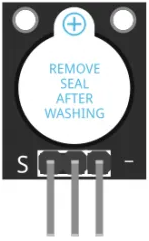
\includegraphics[width=.4\linewidth]{fig/obrazki/buzzer/buzzer2.png}
  \caption{Moduł HW-508 \cite{zdjecia}}
  \label{fig:sub1}
\end{subfigure}%
\begin{subfigure}{.5\textwidth}
  \centering
  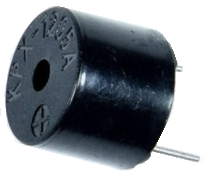
\includegraphics[width=.6\linewidth]{fig/obrazki/buzzer/buzzer_sam.png}
  \caption{Buzzer aktywny \cite{budowa}}
  \label{fig:sub2}
\end{subfigure}
\caption{Przykładowe zdjęcia modułu oraz buzzera}
\label{fig:test}
\end{figure}
\vspace{0.5cm}

Brzęczyki aktywne to rodzaje brzęczyków magnetycznych. Wewnątrz brzęczyka znajduje się cewka z drutu, która jest podłączona do styków brzęczyka. Wokół cewki z drutu znajduje się okrągły magnes. Nad okrągłym magnesem i cewką z drutu znajduje się cienka metalowa folia z przymocowanym na górze metalowym ciężarkiem. Gdy do cewki z drutem są doprowadzane impulsy prądu, indukcyjność magnetyczna powoduje, że metalowy odważnik i metalowa folia drgają w górę i w dół. Drgania folii metalowej powodują powstawanie fal dźwiękowych. Buzzers jest powszechnie stosowany w alarmach, komputerach, drukarkach i innych produktach elektronicznych jako urządzenie dźwiękowe.

\vspace{0.5cm}
\begin{figure}[h]
\centering
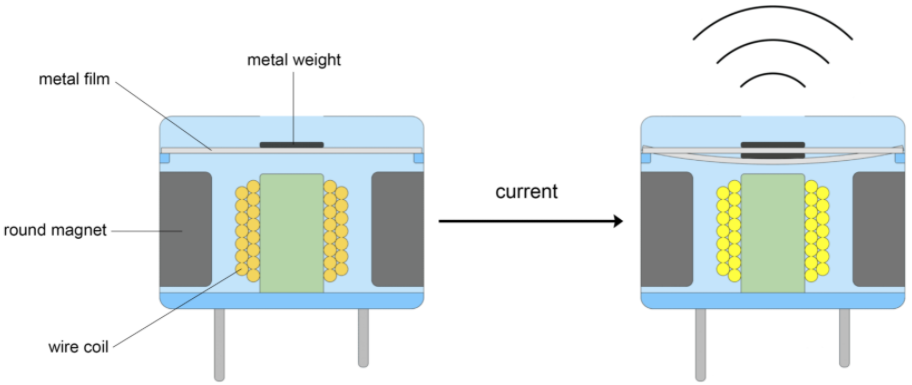
\includegraphics[width=.9\linewidth]{fig/obrazki/buzzer/przekroj.png}
\caption{Przekrój osiowy buzzera \cite{budowa}}
\label{fig:test}
\end{figure}
\vspace{0.5cm}

\section{Użycie czujnika}

\vspace{0.5cm}
\begin{figure}[h!]
    \centering
    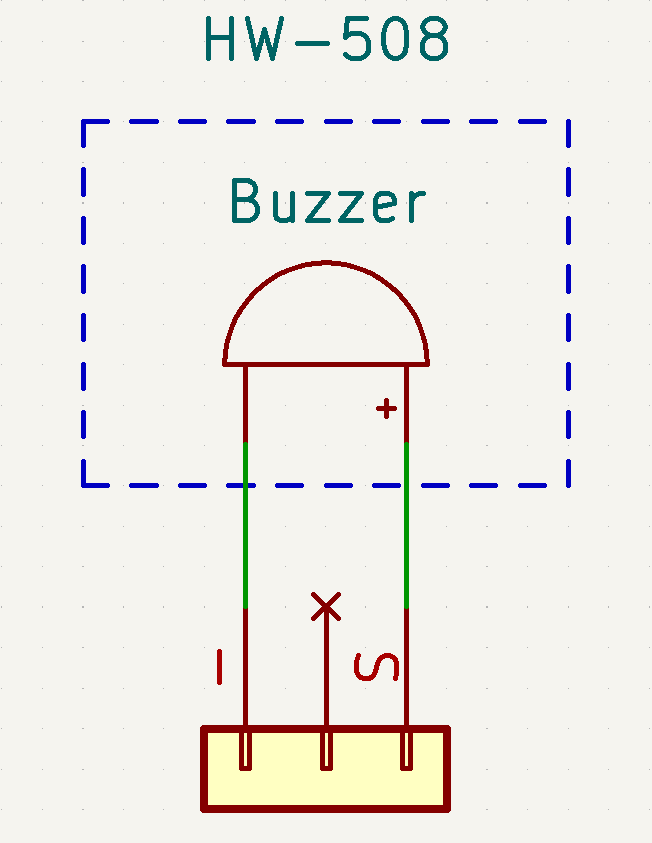
\includegraphics[width=6cm]{fig/obrazki/buzzer/kicadBuzzer.png}
    \caption{Połaczenie elektryczne}
    \label{fig:my_label}
\end{figure}
\vspace{0.5cm}

\section{Prezentacja działania układu}

\vspace{0.5cm}
\begin{figure}[h!]
    \centering
    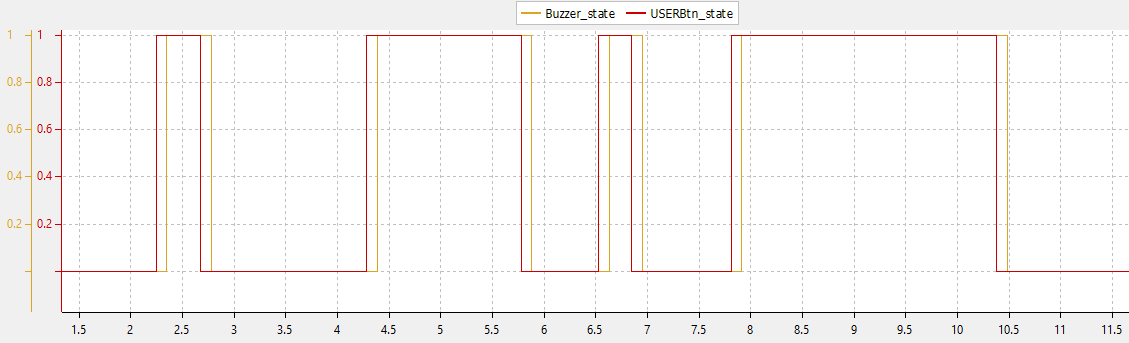
\includegraphics[width=1\textwidth]{fig/obrazki/buzzer/SWVbuzzer.png}
    \caption{Przedstawienie działania układu na wykresie.}
    \label{fig:my_label}
\end{figure}

Jak widać po wciśnięciu przycisku (USERBtn\_state) na wejściu buzzera (Buzzer\_state) pojawia się stan wysoki co powoduje jego brzęczenie (wprowadzone zostało opóźnienie w celu lepszego przedstawienia działania układu).

\newpage

\vspace{0.5cm}
\begin{figure}[h!]
    \centering
    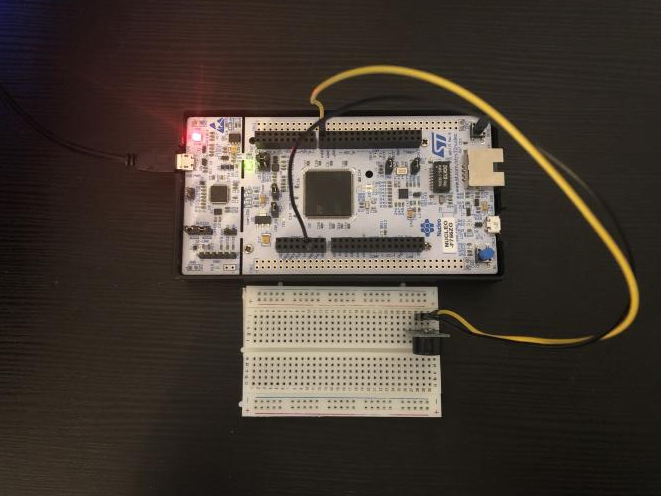
\includegraphics[width=1\textwidth]{fig/obrazki/buzzer/ZdjecieUkladu.png}
    \caption{Zdjęcie układu.}
    \label{fig:my_label}
\end{figure}

Działanie układu zostało jeszcze zaprezentowane na krótkim wideo \cite{youtube}.

\printbibliography[heading=bibintoc]

\end{document}
